% !TEX encoding = UTF-8 Unicode
% !TEX spellcheck = en_US
% !TEX root = ../../../ICMA2020.tex

\subsection{Robot Testbed}
\label{subsec:RobotTestbed}
For experimental evaluations and demonstration of the potential the presented approach was testet on the state-of-the-art serial industrial  robot \textsc{Cloos QRC 350} designed for highly dynamic and precise processes such as assembly or welding tasks, see Fig.\,\ref{fig:testbench}. 
A payload of $10.621\,\mathrm{kg}$ is mounted to the end effector.
The robot is controlled by a standard industrial PLC and servo inverters from the company \textsc{Lenze}. 
For data processing and calculation of the implemented algorithm a desktop computer with \textsc{Matlab} software is used. 
However, in the perspective all calculations can also be carried out directly on the PLC. 
% For a better understanding, the definition of the kinematic parameters $l_1$ -- $l_6$ of the robot are added to this figure.

\begin{figure}[!ht]             % Einbetten in figure wie gehabt
    \centering                  % zentrierte Ausrichtung, optional
    \def\svgwidth{\textwidth/2}    
        % die Bildbreite muss auf diese Weise festgelegt werden!
    %\input{Chapters/Experiments/Robot_Testbed/CLOOS_cover.pdf_tex}  
    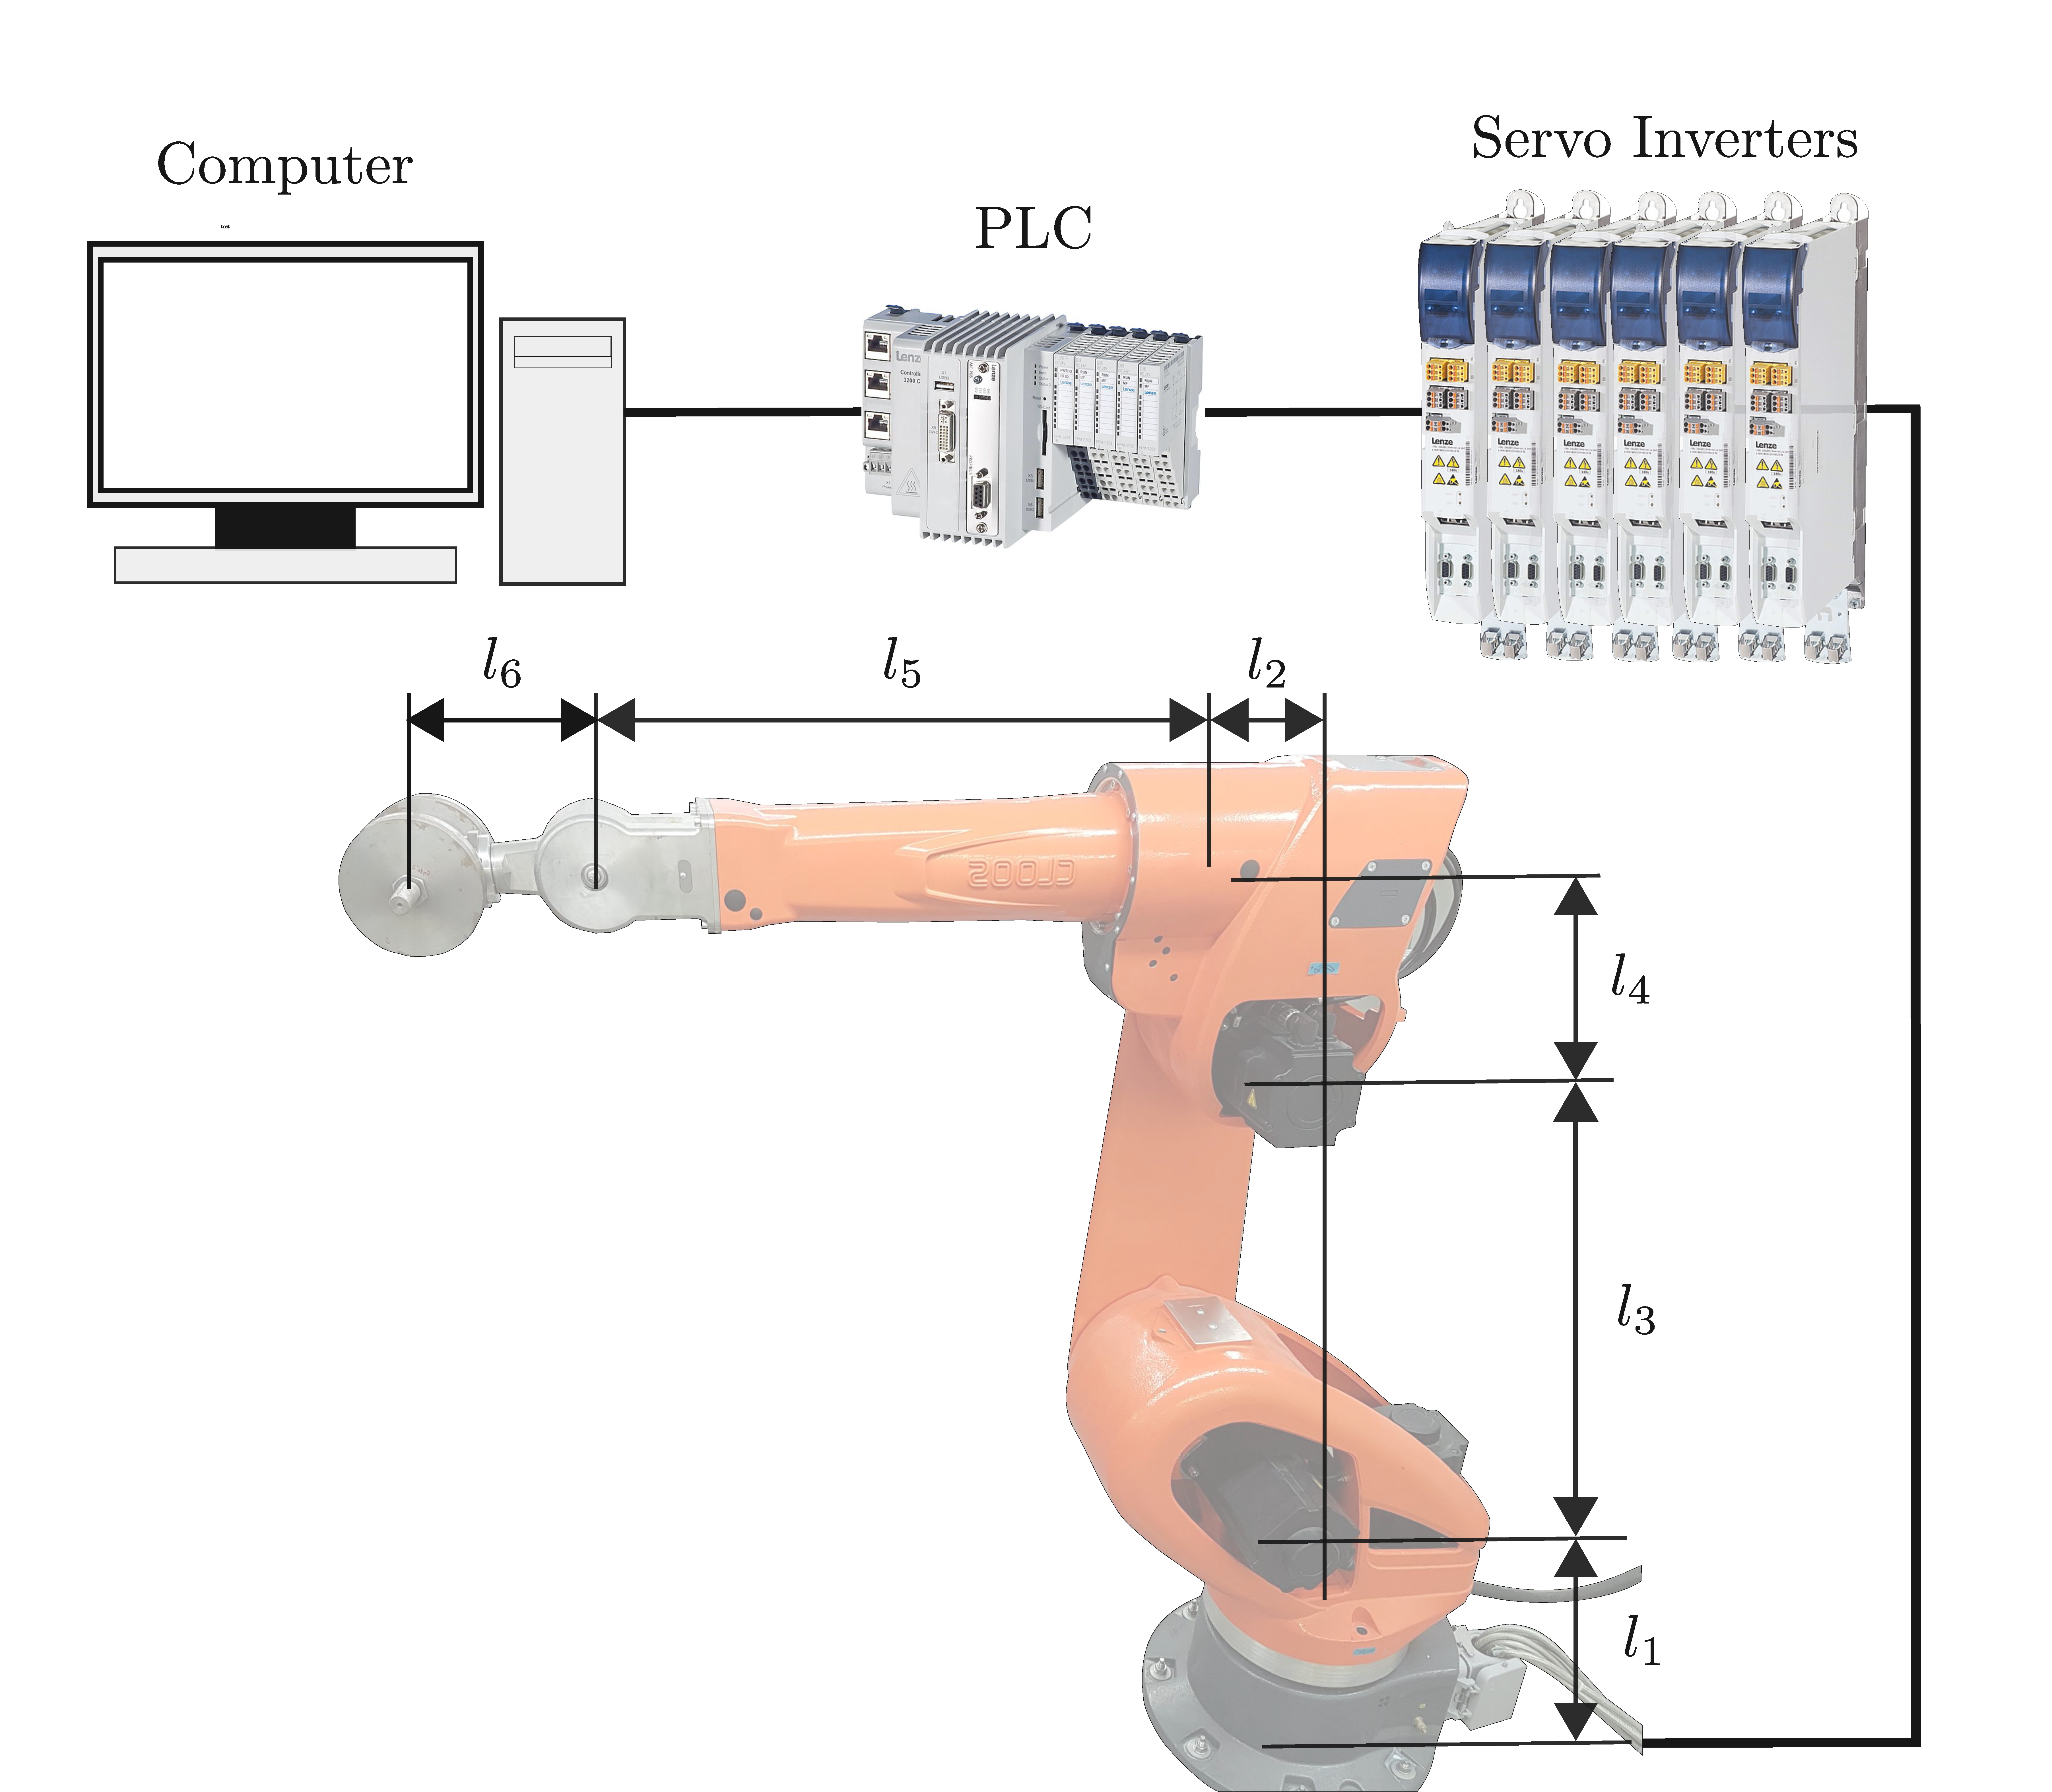
\includegraphics[width=8.6cm]{Chapters/Experiments/Robot_Testbed/Cloos_cover} 
    \vspace{-0.2cm}
    \caption{Experiment setup with a 6-dof \textsc{Cloos QRC 350} industrial robot, PLC and servo inverters and a desktop computer for development.}
    \vspace{-0.2cm}
   \label{fig:testbench}
\end{figure}


% pdf Größe reduzieren mit dem Windows Befehl
%gswin64 -dNOPAUSE -dBATCH -sDEVICE=pdfwrite -dCompatibilityLevel=1.4 -dPDFSETTINGS=/prepress -sOutputFile=prev_events_impressions_small.pdf prev_events_impressions.pdf

% Auflösung: 
%-dPDFSETTINGS=/screen   (screen-view-only quality, 72 dpi images)
%-dPDFSETTINGS=/ebook    (low quality, 150 dpi images)
%-dPDFSETTINGS=/printer  (high quality, 300 dpi images)
%-dPDFSETTINGS=/prepress (high quality, color preserving, 300 dpi imgs)
%-dPDFSETTINGS=/default  (almost identical to /screen)

% Weitere Informationen: http://milan.kupcevic.net/ghostscript-ps-pdf/